\chapter{Analiza wymagań}

Zwracając uwagę na powszechność problemu oraz ilość możliwych parametrów,
które można zmierzyć, stworzony system powinien umożliwiać na obsługę jak 
największej grupy rodzajów odczytów. Zależnie od przeznaczenia użytkownik
powinien mieć możliwość wykorzystania jak największej grupy sensorów ze
zdolnością do wykonywania odczytów różnych parametrów środowiska.
Taka implementacja możliwa jest poprzez stworzenie generycznego rozwiązania, które
nie ograniczałoby użytkownika i na jego podstawie tworzenie oprogramowania
sterującego danym modelem urządzenia.
Może być to osiągnięte z użyciem odpowiednich poziomów abstrakcji w oprogramowaniu.
Umożliwiłoby to również na zwiększoną modularność rozwiązania oraz
wyłączenie niewymaganych w danym zastosowaniu składników systemu.
Dzięki temu zmniejszona zostaje złożoność oraz rozmiar oprogramowania
na urządzeniu monitorującym.

Niektóre sytuacje mogą wymagać reakcji człowieka na zdarzenie, np.
w przypadku niespodziewanego uszkodzenia, którejś z części kontrolującej
temperaturę powietrza. W takich przypadkach dobrym rozwiązaniem jest możliwość
wysyłania powiadomień użytkownikowi o niestandardowym zachowaniu.
Mogą być to informacje o przekroczeniu skonfigurowanej wartości danego czynnika
lub niespodziewanej nagłej jego zmianie. Taki system notyfikacji wraz z
częstym odczytem parametrów może znacznie przyśpieszyć czas reakcji
i naprawy problemu, co może przełożyć się na znacznie zredukowane straty.
Taki system mógłby zostać również wykorzystany do notyfikowania innych
urządzeń o zmianach parametrów tym samym pozwalając na automatyzację
ich działania oraz konfiguracji. Urządzenie mogłoby reagować na daną 
informację i sama dostosować swoje działanie lub w bardziej zaawansowanych
przypadkach logika biznesowa mogłaby znaleźć się po stronie serwera i 
kontrolować pracę tego urządzenia.

Do wielu zastosowań może być również konieczne przeglądanie odczytów historycznych.
Taka funkcjonalność jest konieczna w przypadku, np. badań wpływu danych
parametrów środowiska na badany obiekt. Umożliwia to na ułatwioną korelację
wartości odczytów ze zmianami w podmiocie badań. Przydaje się również 
wraz z wykorzystaniem systemów poprawiających jakość czy temperaturę
powietrza, gdzie porównując wykorzystaną moc urządzenia możemy skorelować
ze zmianami parametrów środowiska wraz z biegiem czasu.
Aplikacja powinna więc mieć możliwość zapisu oraz odczytu danych. Powinny być
one przechowywane w formacie, który umożliwi późniejsze ich łatwe przetwarzanie,
co pomoże w przypadku budowy innych funkcjonalności na zgromadzonych danych
jak również ułatwi samą ich prezentację użytkownikowi. Funkcjonalnością, która
powinna się również pojawić powinna być możliwość filtrowania oraz sortowania
odczytów przez użytkownika.

Ważnym zagadnieniem, które również należy poruszyć jest bezpieczeństwo danych.
W czasach gwałtownie rozwijającego się przemysłu chmur obliczeniowych oraz przechowywania
za ich pomocą danych istotnym jest pochylić się nad potrzebami użytkowników korzystających
z takich rozwiązań. Aplikacja powinna używać zabezpieczonych kryptograficznie protokołów 
jak również udostępnić system uwierzytelniania użytkowników. Pozwoliłoby to konsumentom
takich rozwiązań na wykorzystanie ich w celu wdrożenia tego systemu bez obawy o prywatność
danych.

\section{Wymagania funkcjonalne}
Funkcjonalność aplikacji została podzielona na odpowiednie role użytkowników. 
Każda z nich ma dostęp do odpowiedniego podzbioru funkcji określonych dla ich roli.
Zapewnia to bezpieczeństwo przechowywanych danych oraz uniemożliwia nieautoryzowany dostęp.
\begin{itemize}
  \item \textbf{Urządzenie} ma dostęp do tworzenia odczytów z sensorów oraz połączeń z dedykowanym
    kanałem służącym do przesyłania informacji o statusie oraz konfiguracji. Ich głównym zadaniem
    jest zbieranie informacji o parametrach środowiska, ich przetworzenie do odpowiedniej
    formy, a następnie przesłanie danych w postaci zapytania na serwer. Dodatkowo "zgłaszają"
    swój status serwerowi przy użyciu dedykowanego kanału oraz nasłuchują ewentualnych zmian
    w konfiguracji takiej jak częstotliwość pobierania odczytów. Urządzenie może również
    przejść proces rejestracji - ta akcja tworzy nieaktywne konto, które następnie
    musi zostać zatwierdzone przez administratora, po czym urządzenie jest w stanie
    przesyłać zapytania na serwer.
  \item \textbf{Użytkownik} ma dostęp wyłącznie do podstawowych zasobów aplikacji. Z perspektywy
    tej roli system jest niezmienny - jedyna funkcjonalność dostępna służy pobieraniu danych
    bez możliwości modyfikacji. Są to takie czynności jak pobieranie listy odczytów, ich filtrowanie,
    otrzymywanie notyfikacji oraz przegląd statusu urządzeń. Nie może natomiast tworzyć nowych
    odczytów oraz nie ma dostępu do konfiguracji aplikacji.
  \item \textbf{Administrator} ma dostęp do pełnej funkcjonalności aplikacji. Może wykorzystywać
    wszystkie zasoby dostępne innym rolom. Dodatkowo może modyfikować konfiguracje oraz zarządzać kontami
    innych użytkowników.
\end{itemize}

Funkcjonalność aplikacji została przedstawiona w postaci diagramu przypadków użycia na Rys. \ref{uml:use_case}.
\begin{figure}[h!]
  \centering
  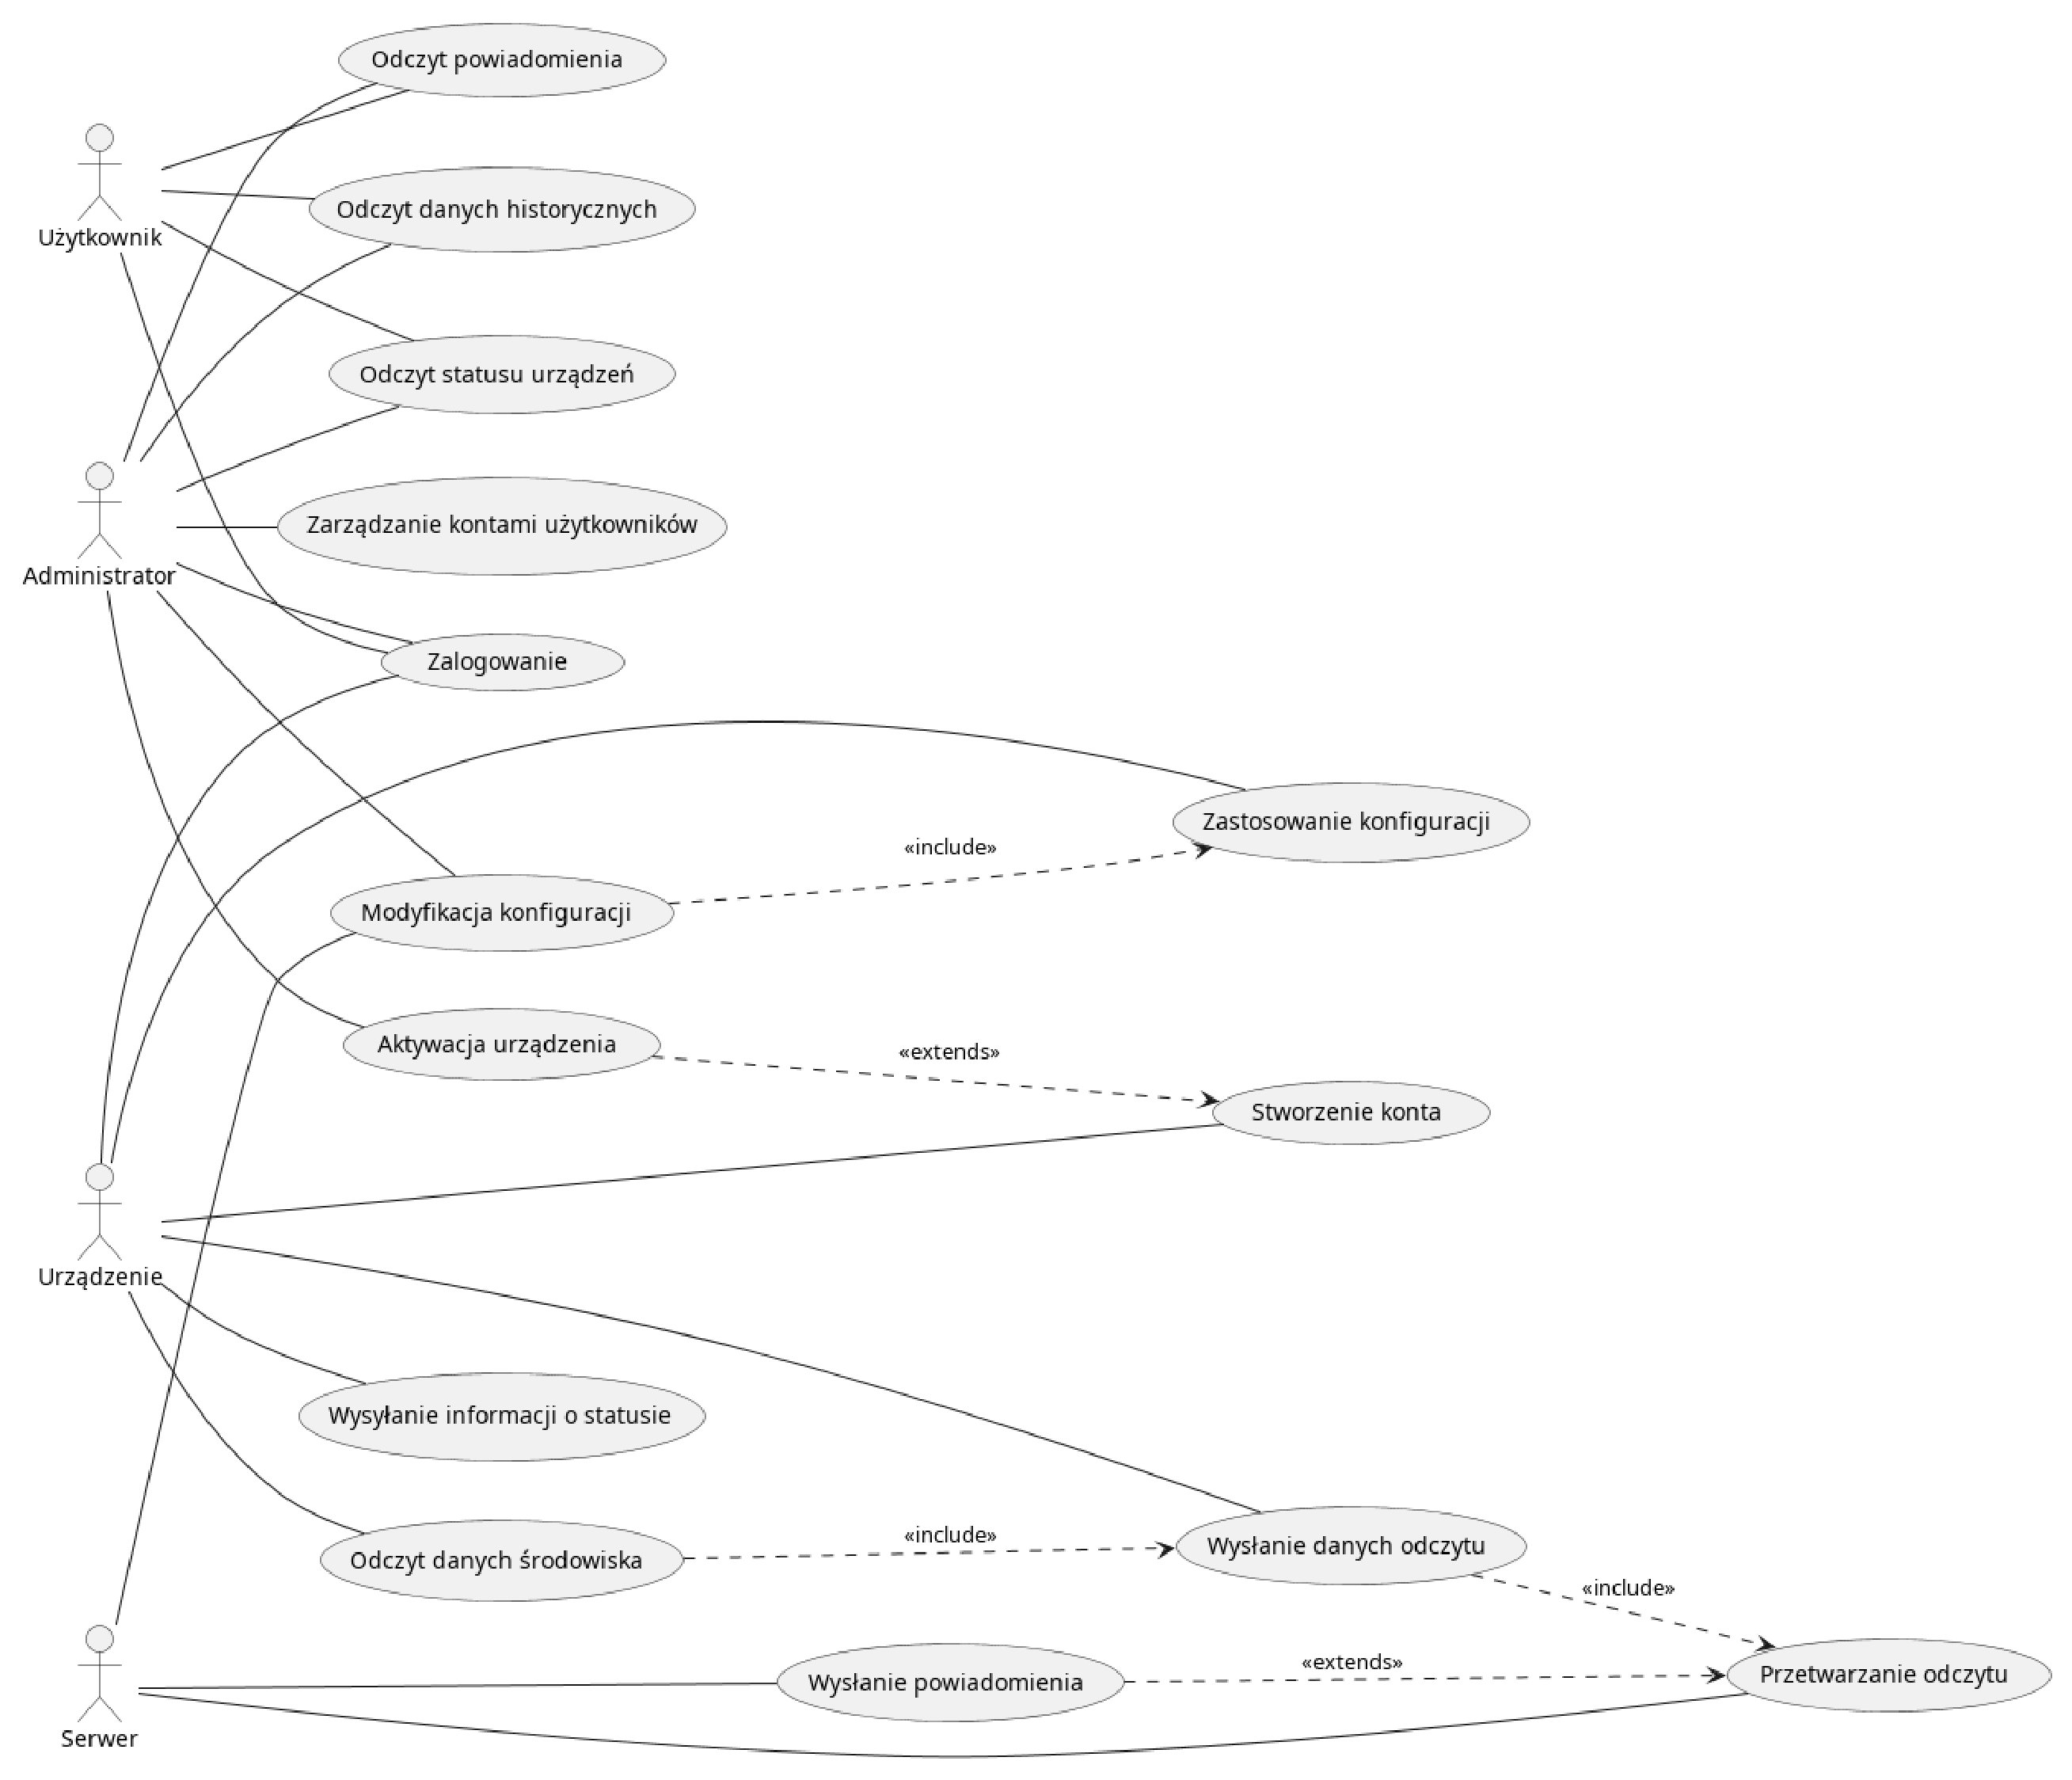
\includegraphics[width=\textwidth]{use_case_diagram}
  \caption{Diagram przypadków użycia}
  \label{uml:use_case}
\end{figure}
Dla lepszego zrozumienia opisane zostały wybrane przypadki użycia.

Pierwszym z nich jest \textbf{odczyt danych środowiska}. W jego wykonaniu uczestniczą aktorzy o roli
urządzenie. Jest ono inicjowane przez urządzenie po upływie, określonego w konfiguracji, przedziału 
czasu od ostatniego tego typu zdarzenia. Wykonywane jest jedynie, gdy urządzenie jest zalogowane w systemie
oraz zostało ono aktywowane przez administratora. Urządzenie w pierwszej kolejności odczytuje wartość
jednego z sensorów po czym przekształca te dane w format przyjmowany przez aplikację serwerową. 
Następnie urządzenie przechodzi do wykonania czynności \textbf{wysłania danych odczytu}. 
W przypadku sytuacji wyjątkowych takich jak niemożliwość odczytu danych z sensora czy brak połączenia
z serwerem dane nie zostają przesłane i urządzenie kontynuuje dalszą pracę. Czynność jest uznana
za zakończoną po odpowiednim sformułowaniu danych i przygotowaniu ich do bycia wysłanymi do aplikacji serwerowej.
Częstotliwość wykonywania tej akcji oraz typowy czas realizacji są narzucone przez konfigurację, lecz w zależności
od ilości przesyłanych danych mogą mieć minimalny czas zależny od sensora.

Kolejnym z nich jest \textbf{przetwarzanie odczytu}. Wykonywane jest przez aktora o roli serwer i jest 
inicjowana po otrzymaniu danych odczytu od aktora urządzenie. Typowo dane po weryfikacji są natychmiastowo
zapisywane w bazie danych. W szczególnych przypadkach, np. brakujących danych serwer zwraca wiadomość
o niepoprawnym zapytaniu, w takim wypadku niekompletne dane nie zostają umieszczone w bazie danych.
Inną sytuacją wyjątkową jest niespełnienie ustalonych przez użytkownika
reguł walidacyjnych - w takim wypadku system przechodzi do czynności \textbf{wysyłanie powiadomienia}, aby
poinformować użytkownika o tym zdarzeniu, następnie system przechodzi do normalnej operacji i zapisuje je
w bazie danych. Końcowym rezultatem tej akcji jest umieszczenie danych odczytu w pamięci stałej oraz
możliwość późniejszego do nich dostępu.

Ostatnim dokładniej opisanym przypadkiem użycia jest \textbf{wysyłanie powiadomienia}. Jest ono wykonywane
przez serwer w przypadku niespełnienia reguł walidacyjnych ustalonych przez użytkownika przez nowy odczyt.
Ma na celu poinformowanie użytkownika o niespodziewanych rezultatach parametrów środowiskowych.
Serwer wysyła powiadomienie z wiadomością skonfigurowaną wcześniej przez administratora. 
Ostatecznym rezultatem tej czynności jest zaprezentowanie użytkownikom oraz administratorom notyfikacji
informującej o danym zdarzeniu.

\section{Wymagania niefunkcjonalne}
Aplikacja została stworzona z myślą o dostępności dla jak największego grona użytkowników.
Przez taki podejście spełnia ona wymagania niefunkcjonalne, które zostały opisane w tym podrozdziale.
\begin{itemize}
  \item Wykorzystane zostały technologie, które są \textbf{otwarto-źródłowe} i/lub stworzone na odpowiedniej
    licencji. Dzięki temu aplikacja jest wolna od dodatkowych kosztów dystrybucyjnych w większości
    przypadków będącym ograniczonym do zawarcia odpowiedniego zapisu w plikach licencyjnych oraz
    udostępnieniu ewentualnych modyfikacji ich kodu źródłowego.
  \item \textbf{Przenośność} była kolejnym aspektem wziętym pod uwagę podczas wyboru technologii. Ważnym jest,
    aby aplikacja mogła być wykorzystana przez jak największą liczbę urządzeń oraz platform. Dlatego też
    użyte technologie umożliwiają na uruchomienie w wielu różnych środowiskach lub w znacznym stopniu to ułatwiają.
  \item Wykorzystane technologie umożliwiły również na zwiększoną \textbf{skalowalność} aplikacji. System może
    obsługiwać wirtualnie nieograniczoną liczbę urządzeń (w rzeczywistości ograniczoną do mocy obliczeniowej serwera)
    oraz środowisko, w którym została stworzona aplikacja serwerowa umożliwia na łatwe rozszerzenie horyzontalne
    systemu poprzez zastosowanie pośrednika z funkcjonalnością równoważenia obciążenia.
  \item \textbf{Bezpieczeństwo danych} było czynnikiem branym pod uwagę przy tworzeniu aplikacji. 
    Możliwe jest to do osiągnięcia poprzez stworzenie systemów uwierzytelniania oraz autoryzacji uniemożliwiających
    dostęp do danych jak i ich modyfikację nieautoryzowanym podmiotom. Dodatkowo powinny zostać zastosowane
    protokoły komunikacji, które umożliwiają kodowanie danych, a co za tym idzie są znacznie odporniejsze
    na nieautoryzowany odczyt niż w przypadku danych przesyłanych w formie tekstowej.
\end{itemize}

